%% If you have any problems using this template, please contact the author: %%
%% Chris Carmona: carmona@stats.ox.ac.uk ; chriscarmona.me %%

\documentclass[aspectratio=169]{beamer}
\usepackage[english]{babel}
\usepackage[utf8]{inputenc} % so we can input characters with accents (e.g. ő)
\usepackage[export]{adjustbox}
\usepackage{tikz}
\usetikzlibrary{babel, scopes, arrows.meta, calc, decorations.pathmorphing, decorations.markings, shapes.geometric}
\usepackage{pgfplots}

%\Star[opt]{r1}{r2}{pos}
\newcommand\Star[4][]{%
\path[#1]  #4 +(0:#2) -- +(45:#3) -- +(90:#2) -- +(135:#3) -- +(180:#2) -- +(225:#3) -- +(270:#2) -- +(315:#3) -- cycle;}

%polstar[opt]{radius}{position}
\newcommand{\polstar}[3][]{
\Star[fill=black,#1]{1*#2}{0.28*#2}{#3}
\Star[#1, fill=white]{0.8*#2}{0.08*#2}{#3}
}
% Syntax: \centerarc[draw options] (x,y) (r, a1, a2) !spaces are important!
\def \centerarc[#1] (#2) (#3,#4,#5)
{\draw[#1] (#2) + ({#3*cos(#4)},{#3*sin(#4)}) arc (#4:#5:#3);}

%\base[options]{texte après}
\newcommand{\base}[2][]{
\draw (0,0) node {\tiny{$\bullet$}};
\draw [thick, .-latex, #1] (0,0) -- (2,0) node[below]{$\vec{e_{x}}$#2};
\draw [thick, .-latex, #1] (0,0) -- (0,2) node[right]{$\vec{e_{y}}$#2};
}

%\bigarrow[options]{scale}{x}{y}
\newcommand{\bigarrow}[4][]{
  \draw [#1] (#3,#4+0.35*#2)-|(1.2*#2+#3,#4+#2)--(2.5*#2+#3,#4+0)--(1.2*#2+#3,#4-#2)|-(#3,#4-0.35*#2)--cycle;
}

\definecolor{dgreen}{RGB}{0,150,0}
\definecolor{lblue}{RGB}{100,100,255}

%\eye[opt]{size}{x}{y}{rotation}
\newcommand{\eye}[5][]% size, x, y, rotation
{   \draw[rotate around={#5:(#3,#4)}, #1] (#3,#4) -- ++(-.5*55:#2) (#3,#4) -- ++(.5*55:#2);
    \draw[#1] (#3,#4) ++(#5+40:.75*#2) arc (#5+40:#5-40:.75*#2);
    % IRIS
    \draw[fill=blue] (#3,#4) ++(#5+55/3:.75*#2) arc (#5+180-55:#5+180+55:.28*#2);
    %PUPIL, a filled arc
    \draw[fill=black] (#3,#4) ++(#5+55/3:.75*#2) arc (#5+55/3:#5-55/3:.75*#2);
}

%\rgb{r}{g}{b} (de 0 à 255)
\newcommand{\rgb}[3]{rgb,255:red,#1; green,#2; blue,#3}

%\tbase[options]{xi}{additional text}
\newcommand{\tbase}[3][]{
\draw [thick, .-latex, #1] (0,0) -- ({2*(cosh(#2)}, {2*sinh(#2))}) node[below]{$\vec{e_{x}}$#3};
\draw [thick, .-latex, #1] (0,0) -- ({2*(sinh(#2)}, {2*cosh(#2))}) node[right]{$\vec{e_{y}}$#3};
}


%\usepackage{Presentation/Presentation_layout}
\usepackage{tikz}
\usetikzlibrary{calc,arrows,fadings, automata, positioning}
\tikzfading[name=fade inside,inner color=red,outer color=blue]
\usepackage{graphicx} % ease graphics management

\usefonttheme[onlymath]{serif}

%\usefonttheme{serif} % change font to allow \textbf{}
\usepackage{amsmath,amsthm,amssymb,mathtools} % for math equations
\usepackage[square,sort,comma,numbers]{natbib} % richer citation
\usepackage{breakcites} % avoid overfull hbox for long cites
\definecolor{kthBlue}{RGB}{25, 84, 166}          % Oxford Blue
\definecolor{bggrey}{RGB}{240, 240, 240}          % Oxford Blue

\usepackage{bm}
\usepackage{media9}

\usecolortheme{beaver}
\setbeamercolor{frametitle}{fg=white,bg=kthBlue}
\setbeamercolor{title}{fg=white,bg=kthBlue}
\setbeamercolor{section in toc}{fg=kthBlue}
\setbeamercolor{background canvas}{bg=bggrey}


\DeclareMathOperator{\newdiff}{d} % use \dif instead
\newcommand{\dif}{\newdiff\!}
\newcommand{\fdif}[2]{\dfrac{\dif #1}{\dif #2}}
\newcommand{\ffdif}[2]{\dfrac{\dif^2 #1}{\dif #2^2}}
\newcommand{\fndif}[3]{\dfrac{\dif^{#3} #1}{\dif #2^{#3}}}

\newcommand{\fpart}[2]{\dfrac{\partial #1}{\partial #2}}
\newcommand{\ffpart}[2]{\dfrac{\partial^2 #1}{\partial #2^2}}
\newcommand{\fnpart}[3]{\dfrac{\partial^{#3} #1}{\partial #2^{#3}}}

\DeclarePairedDelimiter\abs{\lvert}{\rvert}%
\makeatletter
\let\oldabs\abs
\def\abs{\@ifstar{\oldabs}{\oldabs*}}
\newcommand\norm[1]{\left\lVert#1\right\rVert}


%% Information (author, title, etc.) %%


\title[Short Title]{% short title for footer
    \color{white} How did the Ever Given get stuck in the Suez canal
    \vspace{0.5cm}
}

\author{Miguel De Le Court}

\institute{
        \textit{Advanced Computation in Fluid Mechanics}\\
        \textit{DD2365}
        \vspace{0.5cm}
}
\date[Venue and Date]{% short date for footer
   Stockholm, June 2021 
}

%% Content of slides %%
%%%%%%%%%%%%%%%%%%%%
\begin{document}
%%%%%%%%%%%%%%%%%%%%

% Title slide %
{
    \setbeamertemplate{footline}{}
    \setbeamertemplate{headline}{}
    \setbeamercolor{background canvas}{bg = kthBlue}
    \setbeamercolor{normal text}{fg=white}
    \usebeamercolor[fg]{normal text}
    \maketitle
}

%----------------------------%
% Contents slide
%\setbeamertemplate{background canvas}{\begin{tikzpicture} \node[opacity=.1]{\includegraphics[width=\paperwidth]{Figures/Presentation/KTH_camp.png}};\end{tikzpicture}}
% only for the image:
% Conclusions
\begin{frame}{Outline}
    \small
    \tableofcontents
\end{frame}
%----------------------------%

%now include the slides
\setbeamercovered{transparent}
%----------------------------%



% Introduction
%----------------------------%
\section{Introduction}
\subsection{Background and recap of the events}
\begin{frame}{Introduction}
    \framesubtitle{The incident}

    The incident on March 23
    \begin{itemize}
        \item Strong winds and gusts reported, other ships waited due to the bad weather\cite{wind}
        \item Estimated cost of \$9 billion per day
    \end{itemize}

    \begin{figure}
        \centering
        \includegraphics[width=1.05\linewidth, center]{Figures/snaps.pdf}
    \end{figure}
\end{frame}

%----------------------------%

\begin{frame}{Introduction}
    \framesubtitle{The bank effect}

    The bank effect
    \begin{itemize}
        \item Happens due to the high pressure around the bow, low pressure elsewhere
        \item Gives a good qualitative description of the final step
        \item Doesn't explain how we got there
    \end{itemize}

    \begin{center}
    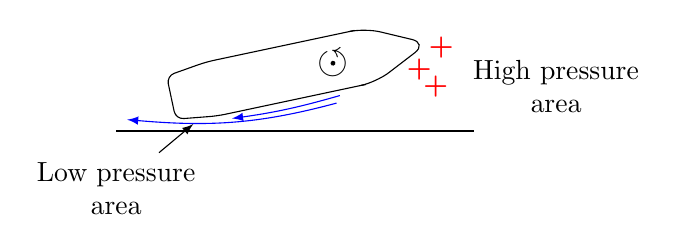
\begin{tikzpicture}[scale=0.7]
        \begin{scope}[shift={(1,0.6)}, rotate=12, scale=0.5]
            \draw[rounded corners=1mm] (0,0)  -- (0, -0.8) -- (1.5,-1) -- (7,-1);
            \draw[rounded corners=1mm] (0,0)  -- (0, 0.8) -- (1.5,1) -- (7,1);
            \draw[rounded corners=2mm] (7, -1) -- (7.4, -1) -- (9.5, 0) -- (7.4, 1)  -- (7,1);
            \draw [blue, -latex] (6, -1.2) to [bend left=4] (2, -1.2);
            \node at (6,0) (P) {\Large $\circlearrowleft$};
            \fill (6, 0) circle[radius=2.5pt];
        \end{scope}
    
        \draw[thick] (0,0) -- (6.5,0);
        \draw [blue, -latex] (4,0.5) to[out=195,in=-5] (0.2,0.2);
        \node[red] at (5.5, 1.1) {$\bm{+}$};
        \node[red] at (5.9, 1.5) {$\bm{+}$};
        \node[red] at (5.8, 0.8) {$\bm{+}$};
        \node[right, align=center] at (6.3, 0.8) (nhp) {High pressure\\ area};
        \node[below, align=center] at (0, -0.4) (nlp) {Low pressure\\ area};
        \draw[-latex] (nlp) -- (1.4,0.12);
    \end{tikzpicture}    
    \end{center}
        
\end{frame}

%----------------------------%
\subsection{State of the art}
\begin{frame}{Introduction}
    \framesubtitle{State of the art}

    ALE models 
    \begin{itemize}
        \item Useful for fluid-structure interaction problems due to its interface capturing capabilities
        \item Problems when the deformations are too large $\longrightarrow$ remeshing
    \end{itemize}

    \vfill    
    Remeshing globally
    \begin{itemize}
        \item Very easy to implement in Dolfin on 1 process
        \item Projected solution introduces a lot of diffusion
        \item Projected flow is not divergence-free $\longrightarrow$ unphysical pressure
    \end{itemize}

    \vfill
    Remeshing locally
    \begin{itemize}
        \item Requires a lower level control on the mesh generation but gives mush better results \cite{Remacle2010May}
    \end{itemize}
\end{frame}

%----------------------------%

\section{Method}
\subsection{Experiments}
\begin{frame}{Method}
    \framesubtitle{Experiments}
    Main goals and experiments:

    \begin{enumerate}
        \setcounter{enumi}{-1}
        \item Get a smooth and accurate movement for the ship in the canal with the corresponding mesh deformation
        \item Simulate the flow while enforcing the movement of the ship, and observe the resulting forces
        \item Reproduce the incident based only on the previously forces, without knowing the path a-priori
        \item Reproduce and try to correct the path by applying a small torque on the ship
    \end{enumerate}
\end{frame}

%----------------------------%

\subsection{Non-dimentionalization}
\begin{frame}{Method}
    \framesubtitle{Non-dimentionalization}
    
    \begin{itemize}
        \item All the computations are base on the non-dimentionnal form of the NS equations 
        \item The scaling factors are $L = 400$m, $U=6$m/s, $\rho = 1000$kg/m$^3$, $\mu=10^{-3}$Pa$\cdot$s $\Longrightarrow R_e = 2.4\times 10^9$
    \end{itemize}

    \vfill
    In this frawemork, Newton's second law can be expressed as 
    \begin{align*}
        \hat{F} &= \dfrac{M_\text{boat}}{M_0} \hat{a} \\
        \hat{\tau} &= \dfrac{M_\text{boat}}{M_0} \hat{I} \hat{\omega}' \\
        M_0 &= L^2 L_c \rho \\
        \hat{I} &= \dfrac{1}{\hat{A}} \int_{\hat{\Omega}_\text{boat}} \dif \hat{A} (\hat{x}^2 + \hat{y}^2)
    \end{align*}



\end{frame}

%----------------------------%

\subsection{The ALE model}
\begin{frame}{Method}
    \framesubtitle{The ALE model}

    \begin{columns}
    \begin{column}{.79\textwidth}
        Boundary conditions on $\bm{u}$
        \begin{itemize}
            \item Dirichlet on the boat and the shore
            \item Neumann on the river
        \end{itemize}
            
        \vspace{0.5cm}
        Boundary conditions on the mesh displacement $\bm{d}$
        \begin{itemize}
            \item Dirichlet on the boat (in $x$ and $y$)
            \item Dirichlet in $x$ on the shore : $\Delta x = 0$, Neumann in $y$
            \item Dirichlet in $y$ on the river : $\Delta y = u_y \Delta t$, Neumann in $x$
            \item Mesh diplacement computed from the historical position or based on the forces
        \end{itemize}


    \end{column}
    
    \begin{column}{.19\textwidth}
    \begin{center}
        
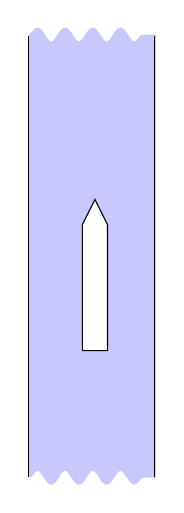
\begin{tikzpicture}[scale=0.4, rotate=90]
    %eau de la rivière
    \draw [thick, fill=\rgb{200}{200}{255}, color=\rgb{200}{200}{255}] decorate [decoration={snake}] {(14,4) -- (14,0)} -- (0,4) decorate [decoration={snake}] {(0,4) -- (0,0)} -- (14,0);

    \path [fill=\rgb{200}{200}{255}] (0.2,0) -- (13.8,0) -- (13.8,4) -- (0.2,4);
    \path [fill=white] (4,1.5) -- (8,1.5) -- (8.8,1.9) -- (8,2.3) -- (4,2.3);
    \draw (4,1.5) -- (8,1.5) -- (8.8,1.9) -- (8,2.3) -- (4,2.3) -- cycle;
    
    %grosses flèches
    %\bigarrow[color=\rgb{150}{150}{255}, fill=\rgb{150}{150}{255}, rounded corners=1mm]{1}{1}{2}
    %\draw [color=\rgb{50}{50}{210}] node at (2,2) {$\vec{v_0}$};
  
    %\bigarrow[color=\rgb{150}{150}{255}, fill=\rgb{150}{150}{255}, rounded corners=1mm]{1}{10}{2}
    %\draw [color=\rgb{50}{50}{210}] node at (11,2) {$\vec{v_0}$};
  
    %les berges noires
    \draw (0,0) -- (14,0);
    \draw (0,4) -- (14,4);
  
    %double flehce cotation evec le "L"
    % \draw [|<->|] (-1,0) -- (-1,4);
    % \draw node [left] at (-1,2) {$L$};
  
    %flèches des parcours
    %\draw [latex-latex, ultra thick, black] (5,0) -- (5,4);
    %\draw [latex-latex, ultra thick, color=\rgb{0}{0}{0}] (5,0) -- (9,0);
  
    %labels des parcours
    %\draw node [rotate=90, left, anchor=south, black] at (5,2) {Parcours $A$};
    %\draw node [above, color=\rgb{0}{0}{0}] at (7,0) {Parcours $B$};
  
    %triangle à droite
    %\draw [thick] (16,0) |- (18,4) --cycle;
    %\draw node [above] at (17,4) {$v_0$};
    %\draw node [left] at (16,2) {$v_a$};
    %\draw node [right] at (17,2) {$c$};
  \end{tikzpicture}
  
    \end{center}
    \end{column}
    \end{columns}
\end{frame}

%----------------------------%

\begin{frame}{Method}
    \framesubtitle{The ALE model}
    Mesh generation
    \begin{itemize}
        \item Dolfin's \texttt{mshr}'s cells were way too small $\longrightarrow$ unusable
        \item Current imlpementation \texttt{gmsh} : good control but slow mesh generation due to the various intermediate formats
    \end{itemize}

    \vfill
    Remeshing criteria
    \begin{itemize}
        \item Mesh quality is too low $(<0.2)$
        \item Some cells become too large
        \item There should be a change in the topology
    \end{itemize}
\end{frame}

%----------------------------%

\subsection{Remeshing problems}
\begin{frame}{Method}
    \framesubtitle{Remeshing problems}
    \begin{columns}
        \begin{column}{.79\textwidth}
            The global remeshing problem
            \begin{itemize}
                \item Remeshing causes very strong pressure oscillations for a few iterations
                \item If nothing is done, it renders the rest of the computation meaningless
                \item The instability only lasts for about $\approx 15$ iterations, regardless of $\Delta t$
            \end{itemize}
            \vspace{0.2cm}
            Implemented solution
            \begin{itemize}
                \item Compute 15 iterations with $\Delta t = \Delta t_0/15$
                \item Add a strong smoothing effet in the force computation after a remesh for $\approx 20$ iterations
            \end{itemize}
    
    
        \end{column}
        
        \begin{column}{.1\textwidth}
            \begin{figure}
                \centering
                \adjincludegraphics[height=6cm,trim={2.2cm 7cm 2.44cm 7cm},clip]{Figures/img00298.jpg}
            \end{figure}
        \end{column}
        \begin{column}{.1\textwidth}
            \begin{figure}
                \centering
                \adjincludegraphics[height=6cm,trim={2.2cm 7cm 2.44cm 7cm},clip]{Figures/img00299.jpg}
            \end{figure}
        \end{column}
    \end{columns}
    
\end{frame}

%----------------------------%
\subsection{Applying the force}
\begin{frame}{Method}
    \framesubtitle{Applying the force}
    Application of the force
    \begin{itemize}
        \item Done strongly, using the Crank-Nicolson method
        \item Still unstable without smooting, even whith an implicit method
        \item We use $\tilde{F}$, such that $\tilde{F}_{i+1} = (1-w) \cdot \tilde{F}_i + w \cdot F_\text{computed}$
        \item     The computation is still sensitive in the choice of $\Delta t$, the reasons will become aparent in the results
    \end{itemize}
    
    \vfill
    Decomposition forces
    \begin{itemize}
        \item Engine : in the direction of the ship
        \item Extrenal forces : computed from the fluid forces, the engine force, and the acceleration
    \end{itemize}


\end{frame}

%----------------------------%


\section{Results}
\subsection{Path enforced}
\begin{frame}{Results}
    \framesubtitle{Path enforced}

    \begin{figure}
        \centering
        \includegraphics[width=1.1\linewidth, center]{Figures/forces.pdf}
        \caption{Forces exerted on the ship in comparison with the forces needed to achieve the observed acceleration}
        \label{fig:forces}
    \end{figure}
\end{frame}

%----------------------------%

\begin{frame}{Results}
    \framesubtitle{Path enforced}
    \begin{itemize}
        \item The lateral forces and the torque are an order of magnitude greater than expected
    \end{itemize}

    \begin{figure}
        \centering
        \includegraphics[width=1.1\linewidth, center]{Figures/forces_wrong.pdf}
    \end{figure}
\end{frame}

%----------------------------%

\subsection{Path from the computed force}
\begin{frame}{Results}
    \framesubtitle{Path from the computed force}

    \begin{itemize}
        \item Path from the forces is surprisingly accurate
    \end{itemize}

    \begin{figure}
        \centering
        \includegraphics[width=1.1\linewidth, center]{Figures/simu_snaps.pdf}
    \end{figure}
\end{frame}

%----------------------------%

\subsection{Corrected path}
\begin{frame}{Results}
    \framesubtitle{Corrected path}

    \begin{itemize}
        \item The forces we had to face hare are much greater than in reality
        \item We were still able to avoid the incident with only minor torque changes $(\abs{\hat{\tau}_\text{added}} \leq 0.02)$
    \end{itemize}

    \begin{figure}
        \centering
        \includegraphics[width=1.1\linewidth, center]{Figures/simu_correct_snaps.pdf}
    \end{figure}
\end{frame}

%----------------------------%

\section{Discussion}
\subsection{The problem of the lateral force}
\begin{frame}{Discussion}
    \framesubtitle{The problem of the lateral force}
    Longitudinal force
    \begin{itemize}
        \item Is consistently pointing backwards with a magnitude of $\hat{F} = 0.0375 \Leftrightarrow 7500kN$
        \item Translates to $45$MW of power : consistent with $60$MW engine
    \end{itemize}

    \vfill
    Lateral force
    \begin{itemize}
        \item Way too large to be explained by external factors such as wind (450km/h)
        \item Probably due to the 2D model : there should be a path below the ship
    \end{itemize}
\end{frame}

%----------------------------%

\begin{frame}{Discussion}
    \framesubtitle{The consequences of the lateral force}
    
    \begin{itemize}
        \item Causes the torque to be all over the place
        \item Bank effects are also overestimated 
        \item A different $\Delta t \Longrightarrow$ slightly different paths $\Longrightarrow$ slightly different forces $\Longrightarrow$ very different lateral forces $\Longrightarrow$ more different path... : explains the sensitivity of the second and third simulations to the choice of $\Delta t$
    \end{itemize}
\end{frame}

%----------------------------%

\subsection{Corrected path}
\begin{frame}{Discussion}
    \framesubtitle{Corrected path}
    
    Observations from the corrected path simulations
    \begin{itemize}
        \item Possible to avoid the incident with minimal input, even with the massively overstimated side forces
        \item Positive feedback loops happen while turing, in some situations
        \item Many times, the best input is very counter-intuitive
    \end{itemize}
\end{frame}

%----------------------------%

\section{Conclusion}
\begin{frame}{Conclusion}
    \begin{itemize}
        \item Experiments failed to provide a good quantitative description of the forces during the events
        \item Gives, however, a good qualitative description of the dynamics of the canal blocking
        \item Avoiding the incident was possible but predicting the right command beforehand is hard and maybe not possible without insight into the future
    \end{itemize}
\end{frame}

%----------------------------%

\subsection{Future work and possible improvements}
\begin{frame}{Conclusion}
    \framesubtitle{Future work and possible improvements}
    
    Improvements of the remeshing
    \begin{itemize}
        \item Use a localized remeshing, to greatly increase the robustness
        \item Use a different kind of projection that preserves a divergence-free $\bm{u}$
    \end{itemize}

    \vfill
    Side forces
    \begin{itemize}
        \item Use a 3d model
        \item model the ship as a porous media
    \end{itemize}
\end{frame}

%----------------------------%

\begin{frame}{Conclusion}
    \vfill
    \begin{center}
        \large Thank you
    \end{center}
    \vfill
    \begin{center}
        \large Questions are welcome
    \end{center}
    \vfill
\end{frame}

%----------------------------%




\begin{frame}
    \frametitle{References}
    \footnotesize
    \bibliographystyle{IEEEtran}
    \bibliography{biblio.bib} % bibliography file
\end{frame}
    


%%%%%%%%%%%%%%%%%%%%
\end{document}
%%%%%%%%%%%%%%%%%%%%
